\subsection{Dijet Measurements}
\label{sec:res_dijet}

The principles of the dijet asymmetry method for the measurement
of the jet \pt resolution were presented in Section~\ref{sec:methods}. Here, the results of the measurement are presented.

The idealized topology of two jets with exactly compensating
transverse momenta is spoiled in realistic collision events by the
presence of extra activity, e.g. from additional soft radiation or from
the UE. The resulting asymmetry distributions are broadened and
the jet \pt resolution is systematically underestimated.
Other effects can also cause jet imbalance.
For example, fragmentation effects cause some energy to be
showered outside the jet cone (``out of cone radiation'').
The width of the asymmetry distribution is thus a convolution of
these different contributions:

\begin{equation}
\sigma_\mathcal{A} = \sigma_{intrinsic}\oplus\sigma_{imbalance}
\label{eq:convolution}
\end{equation}

To account for soft radiation in dijet events,
the measurement of the asymmetry in each $\eta$ and
$\ptave$ bin is carried out
multiple times, for decreasing amounts of extra activity, and the jet \pt
resolution is extracted by extrapolating the extra event activity to zero,
as discussed in Section \ref{sec:radbias}.
The ratio of the transverse momentum of the third jet in the event over
the dijet average \pt, $\pt^{Jet3, rel}=\ptrelthree$, is used as a measure of
the extra activity.
The extrapolation procedure is illustrated in
Fig.~\ref{fig:extrap-example} (left) for the
$120 < \ptave < 147\GeV$ bin of PF jets
and for the corresponding bin of MC particle jets (right).
The width of each asymmetry distribution $\sigma_\mathcal{A}$, as well as the resolutions obtained
using generator-level MC information, are derived based on the RMS of the
corresponding  distributions.
Some characteristic example distributions for the raw asymmetry are shown
for PF jets in Fig.~\ref{fig:asym-mcdata-pf-eta00to05}.
\begin{figure}[h]
\centering
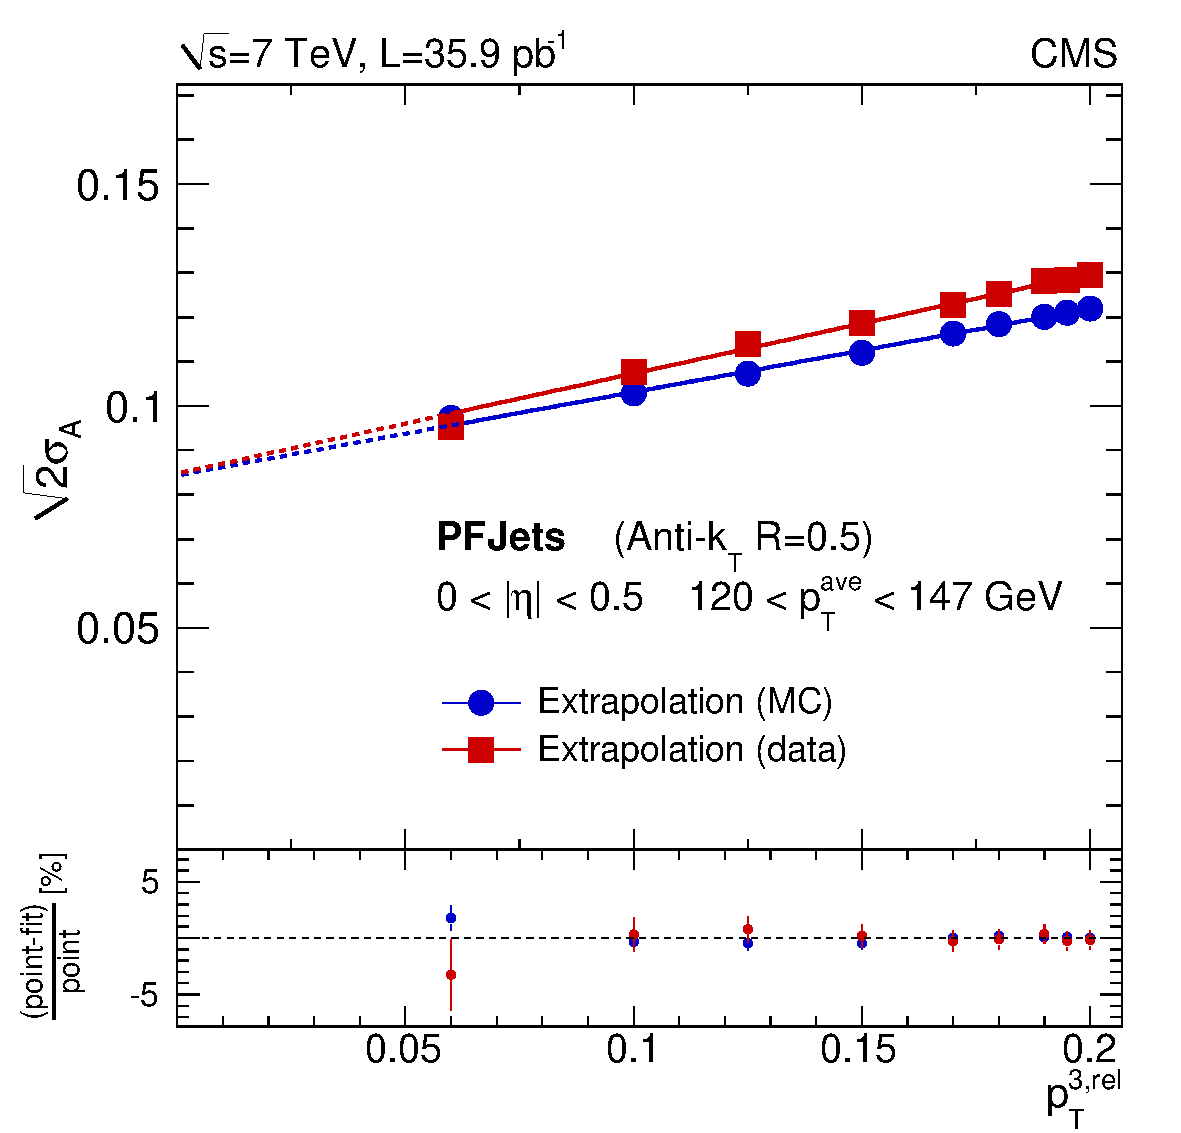
\includegraphics[width=0.49\textwidth]{Figures/JER/figs/res_dijet/ak5pf_AsymVsThreshPt_JetEta0to0dot5_RefPt120to147}
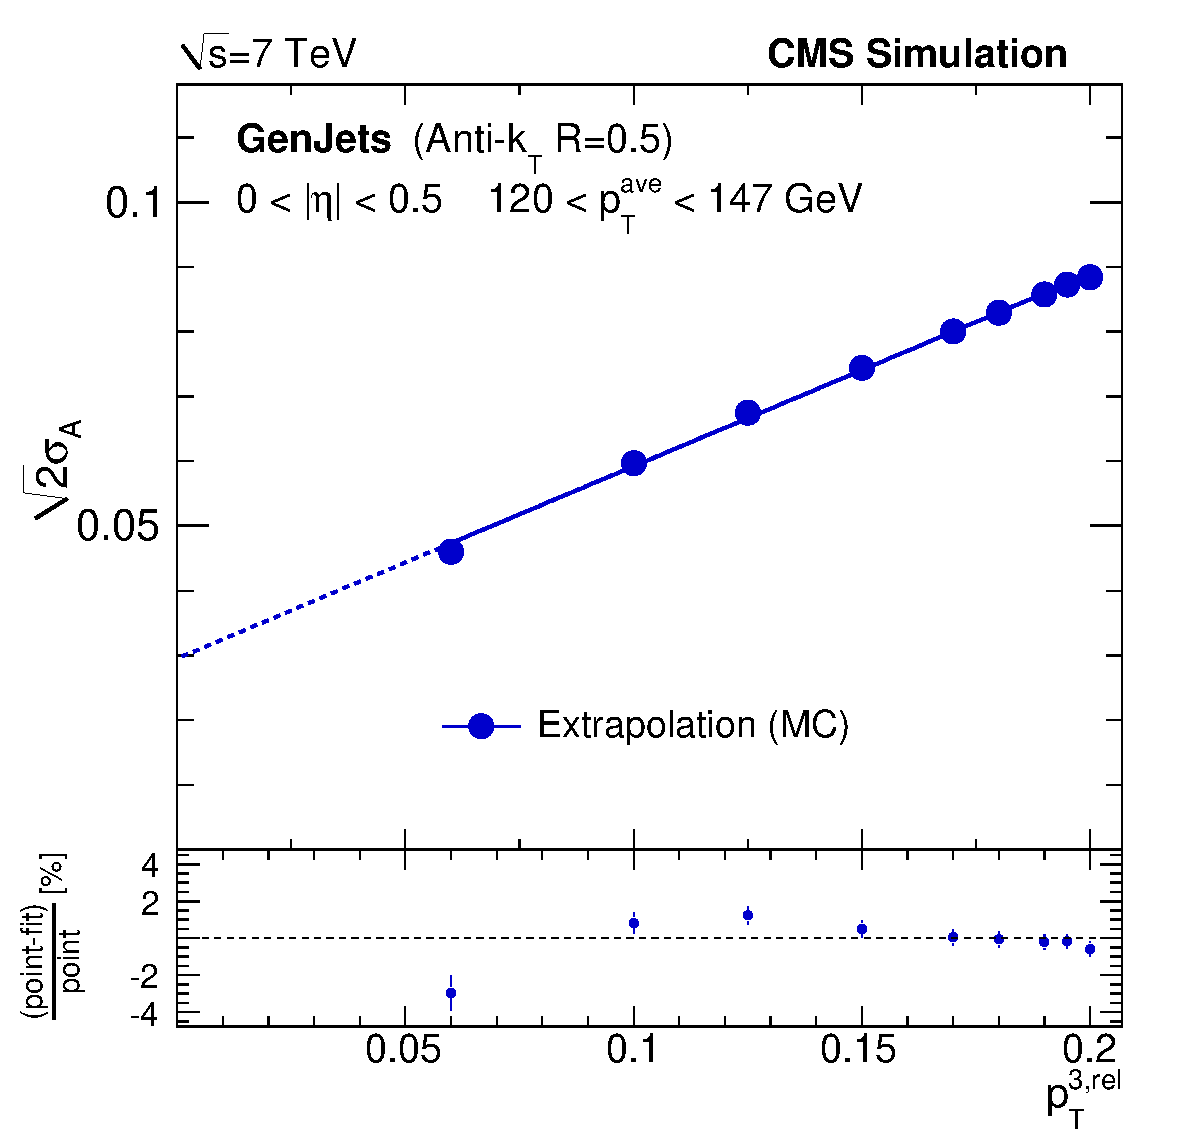
\includegraphics[width=0.49\textwidth]{Figures/JER/figs/res_dijet/gen_AsymVsThreshPt_JetEta0to0dot5_RefPt120to147}

  \caption{Examples of extrapolations of $\sqrt{2}\sigma_\mathcal{A}$
   as a function of
  \ptrelthree to zero for PF jets ($R=0.5$) in $|\eta|<0.5$ and $120<\ptave<147\GeV$ (left).
  Example of a corresponding extrapolation  for MC particle jets (right).}
\label{fig:extrap-example}
\end{figure}

\begin{figure}[h]
\centering
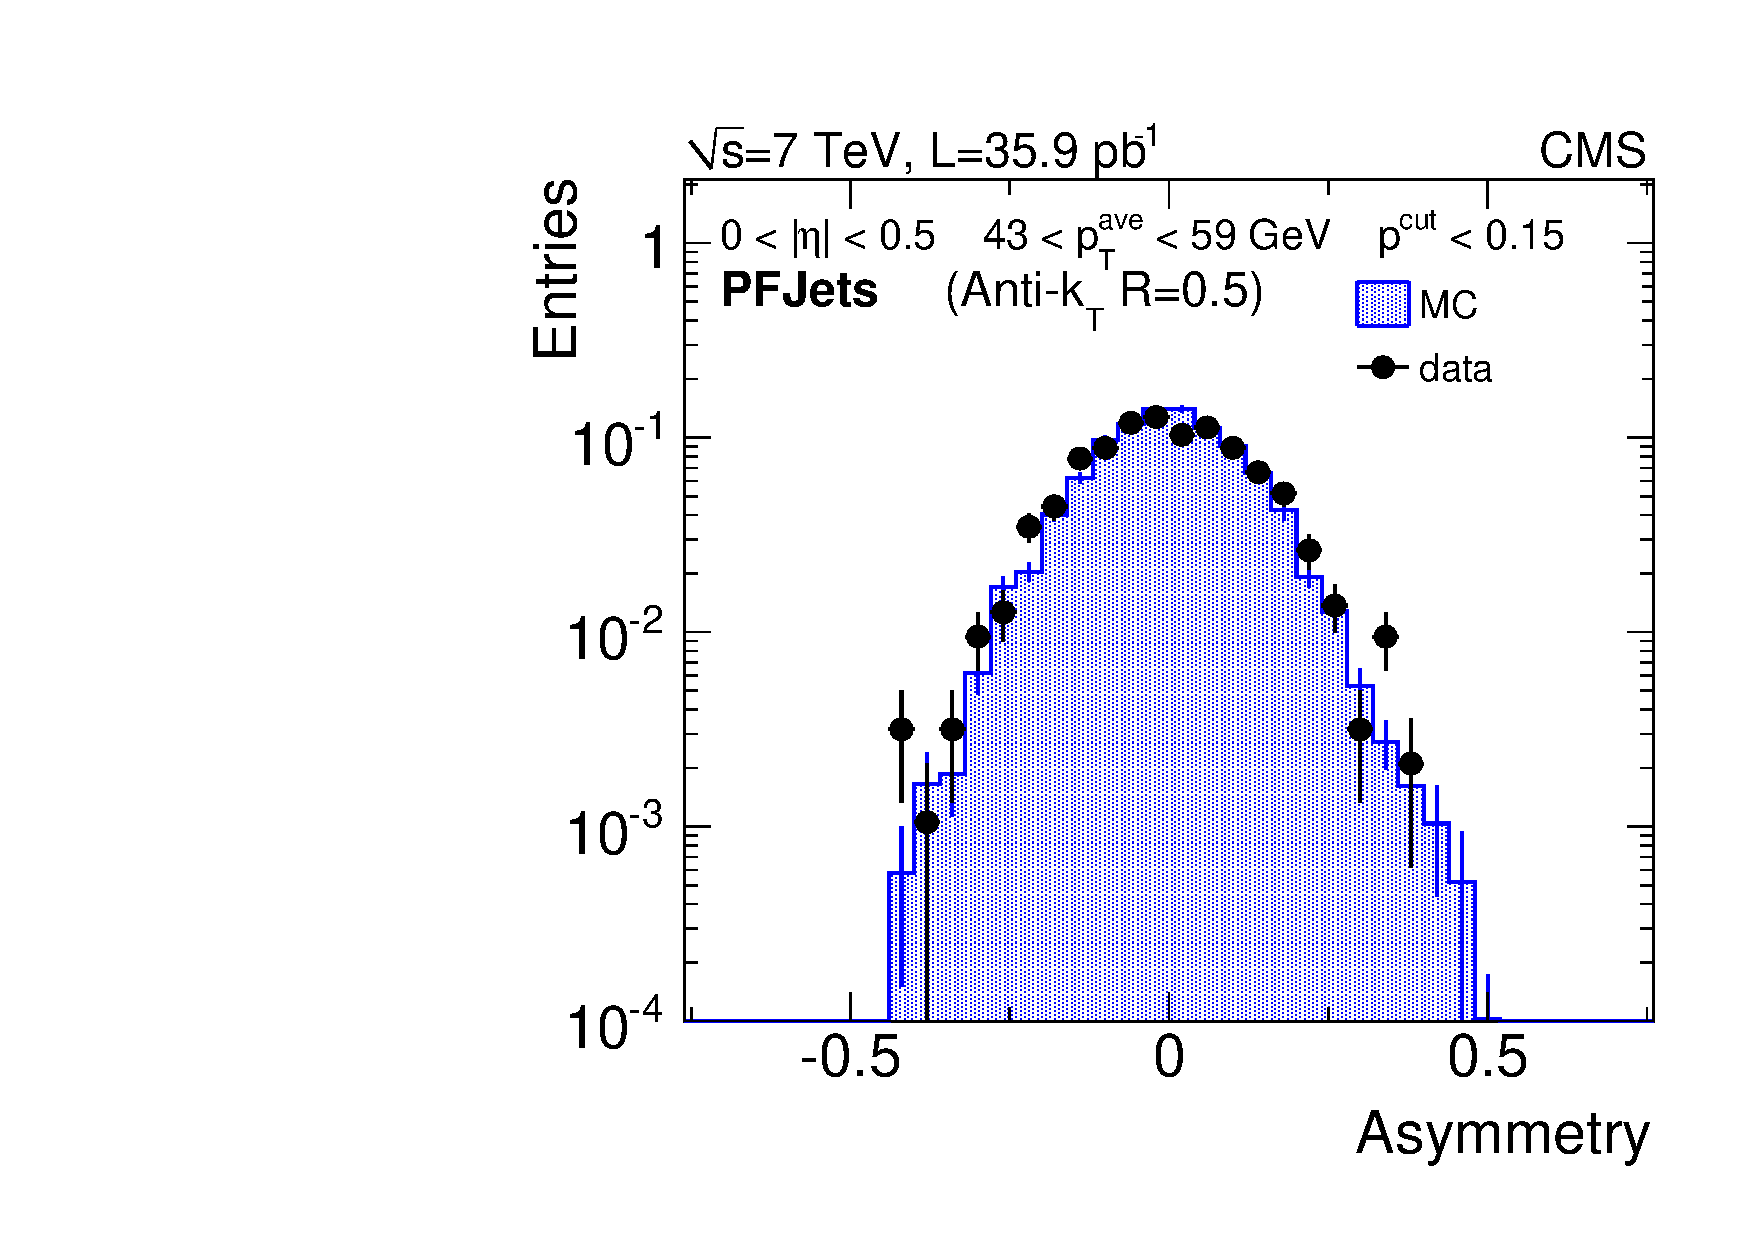
\includegraphics[width=0.45\textwidth]{Figures/JER/figs/res_dijet/ak5pf_Asym_JetEta0to0dot5_RefPt43to59_ThreshPt0dot125to0dot15}
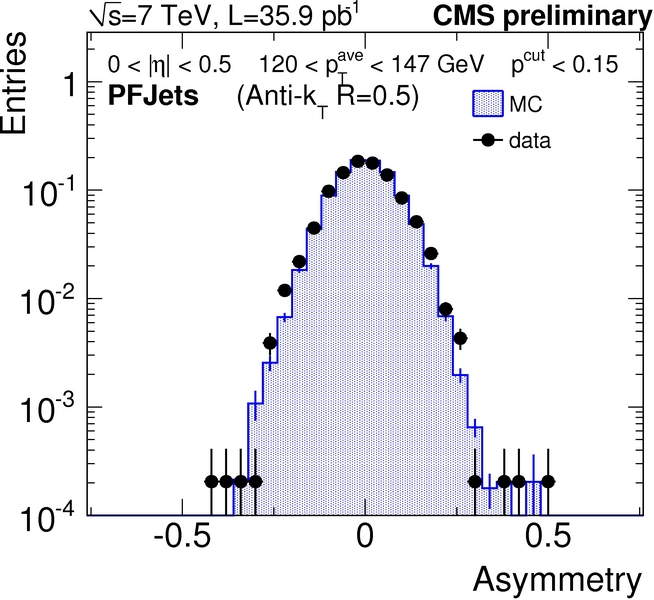
\includegraphics[width=0.45\textwidth]{Figures/JER/figs/res_dijet/ak5pf_Asym_JetEta0to0dot5_RefPt120to147_ThreshPt0dot125to0dot15}
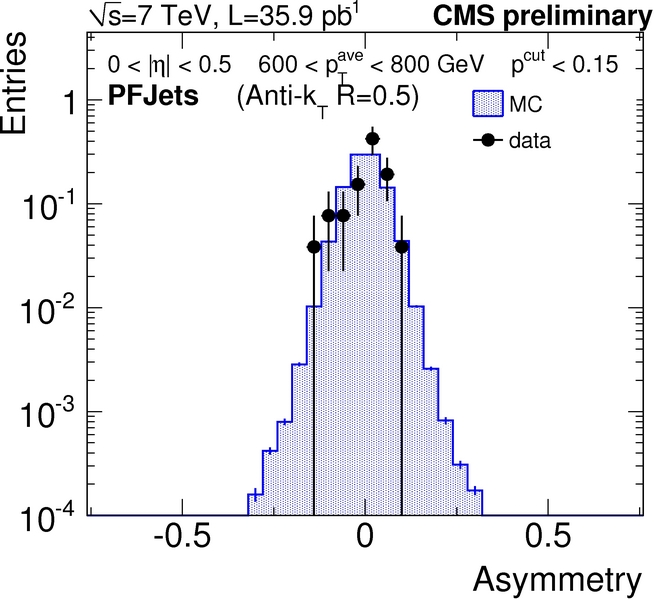
\includegraphics[width=0.45\textwidth]{Figures/JER/figs/res_dijet/ak5pf_Asym_JetEta0to0dot5_RefPt600to800_ThreshPt0dot125to0dot15}
\caption{Examples of PF jet asymmetry distributions for $|\eta|<0.5$ and a low-\ptave bin (top left), a medium-\ptave bin (top right) and a high-\ptave bin (bottom), determined from QCD simulation (blue histograms) and compared with the result from data (black dots).}
\label{fig:asym-mcdata-pf-eta00to05}
\end{figure}

To account for the particle-level imbalance contribution to the measured jet \pt resolution, the asymmetry method is applied to the generated MC particle jets. Then the extrapolated particle-level resolution is subtracted in quadrature from the measurement.
Figure~\ref{fig:reso-mc-00to05} illustrates the different steps of the asymmetry procedure for CALO, JPT, and PF jets respectively.
The total \pt resolution derived from the extrapolation of the reconstructed asymmetry is shown in green circle, the estimation of the particle-level imbalance resolution from the application to MC particle jets is shown in magenta diamond, and the quadrature subtraction to the final asymmetry result is shown in blue square. All three can be described by a fit to a variation of the standard
formula for calorimeter-based resolutions,

\begin{equation}
  \frac{\sigma(\pt)}{\pt} =
  \sqrt{\mathrm{sgn}(N)\cdot\left(\frac{N}{\pt}\right)^2+S^2\cdot
    \pt^{(M-1)}+C^2},
\end{equation}

where, $N$ refers to the "noise", $S$ to the "stochastic",
and $C$ to the "constant" term. The additional parameter $M$ is
introduced, and the negative sign of the noise term is allowed,
to improve the fits to the jet \pt resolution vs. \pt,
for jets that include tracking information (JPT, PF),
while retaining a similar functional form as
the one used for CALO jets. The resolution estimated from  generator-level
MC information is shown in red triangles, and good agreement with the result
of the  asymmetry method is observed. The ratio
$\mathrm{\frac{MC(generator-level)}{MC(asymmetry)}}$ is obtained as a
function of \pt, for each jet type and in each $\eta$-bin and is later
applied to the data measurement as a bias correction.

\begin{figure}[h]
  \centering
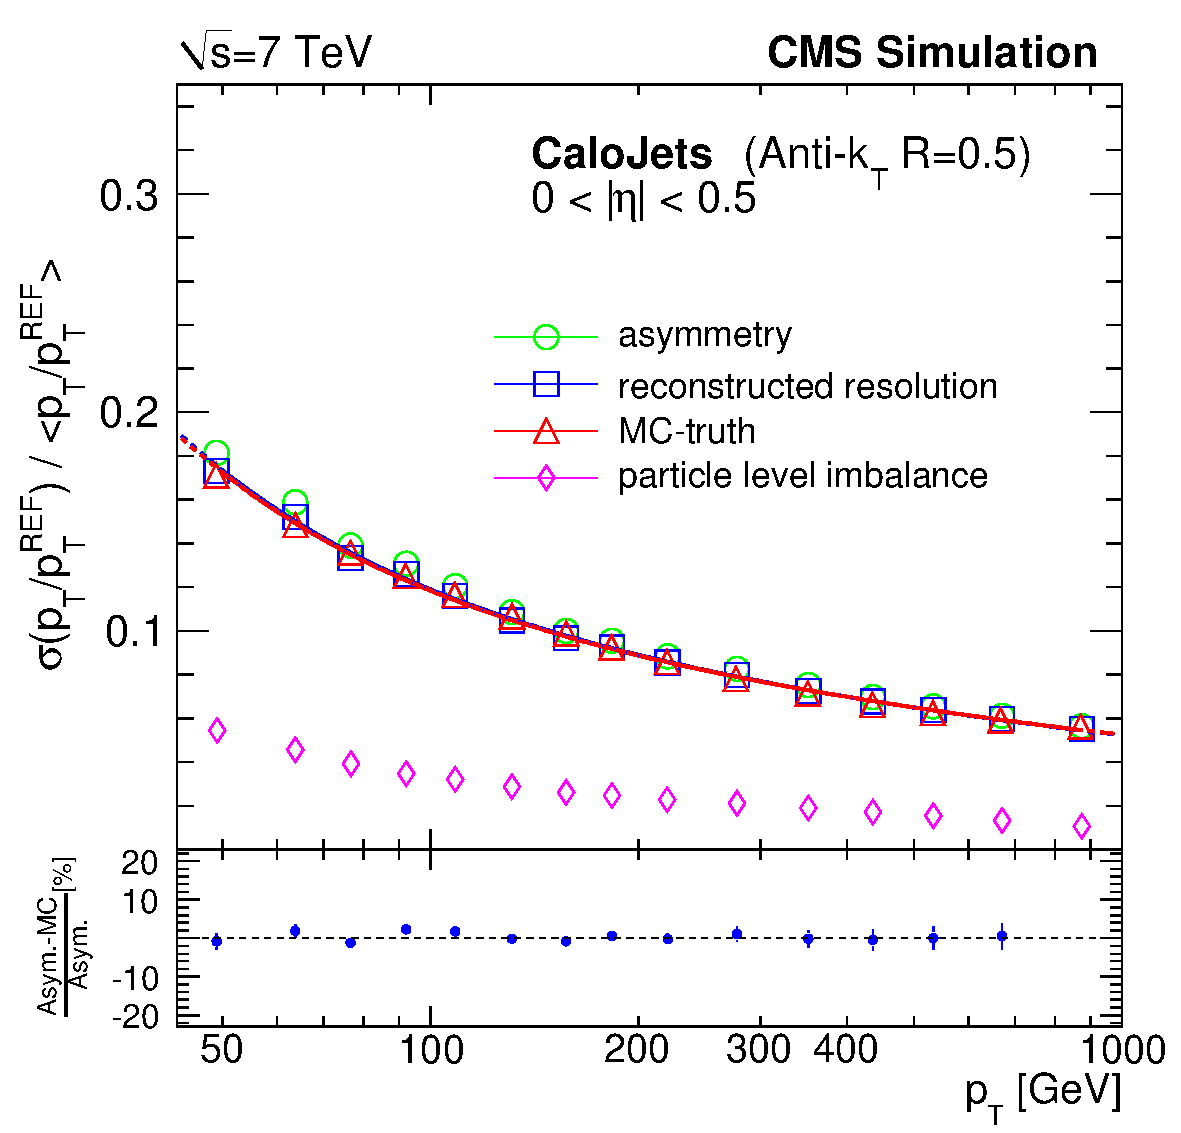
\includegraphics[width=0.45\textwidth]{Figures/JER/figs/res_dijet/ak5calo_mctruth_RelResVsRefPt_JetEta0to0dot5}
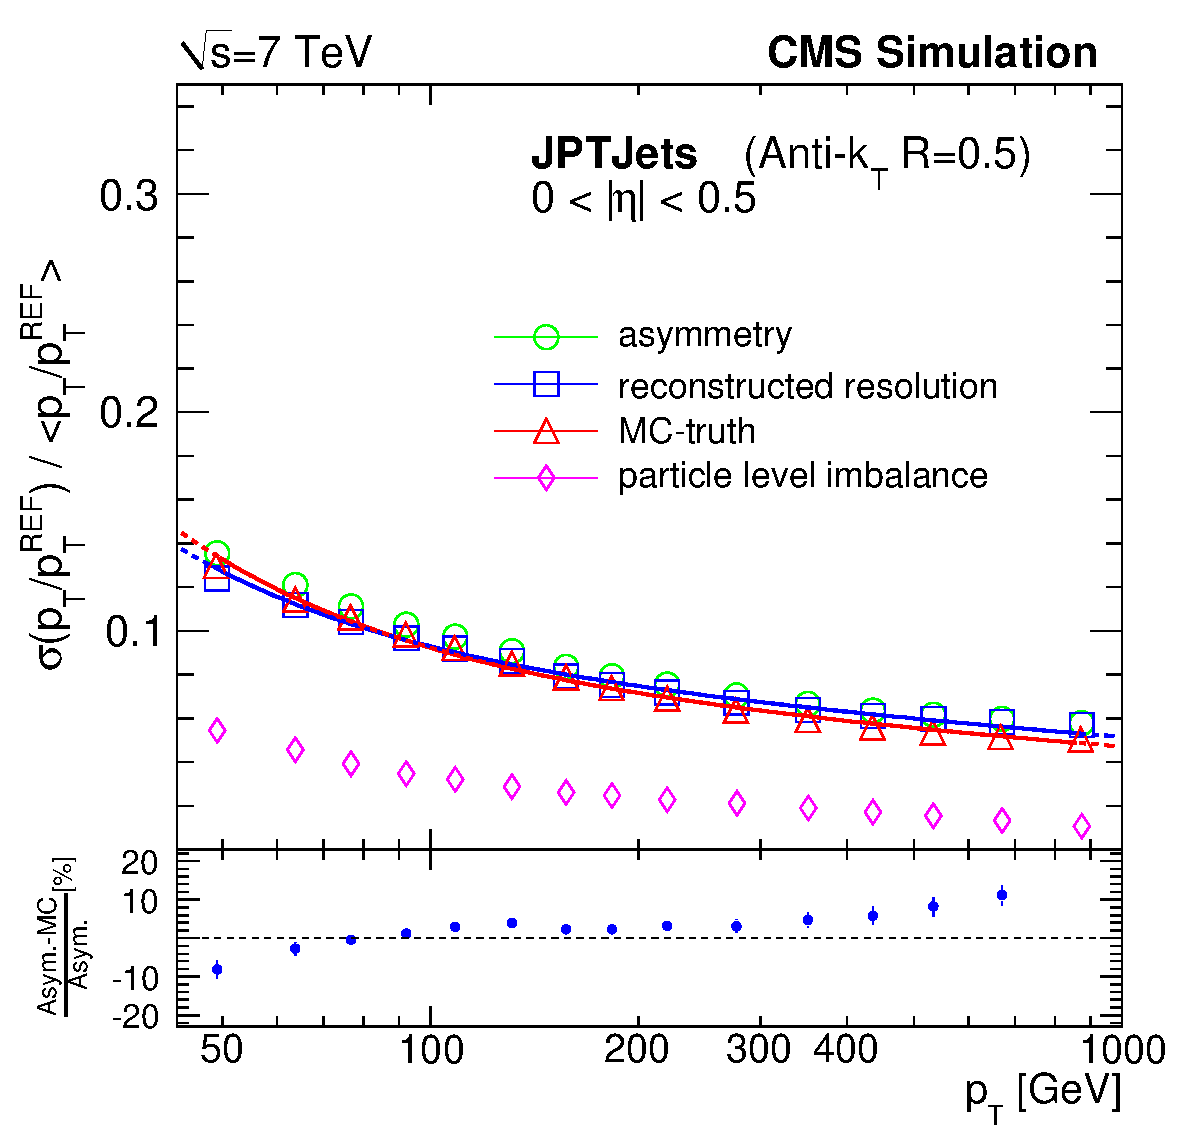
\includegraphics[width=0.45\textwidth]{Figures/JER/figs/res_dijet/ak5jpt_mctruth_RelResVsRefPt_JetEta0to0dot5}
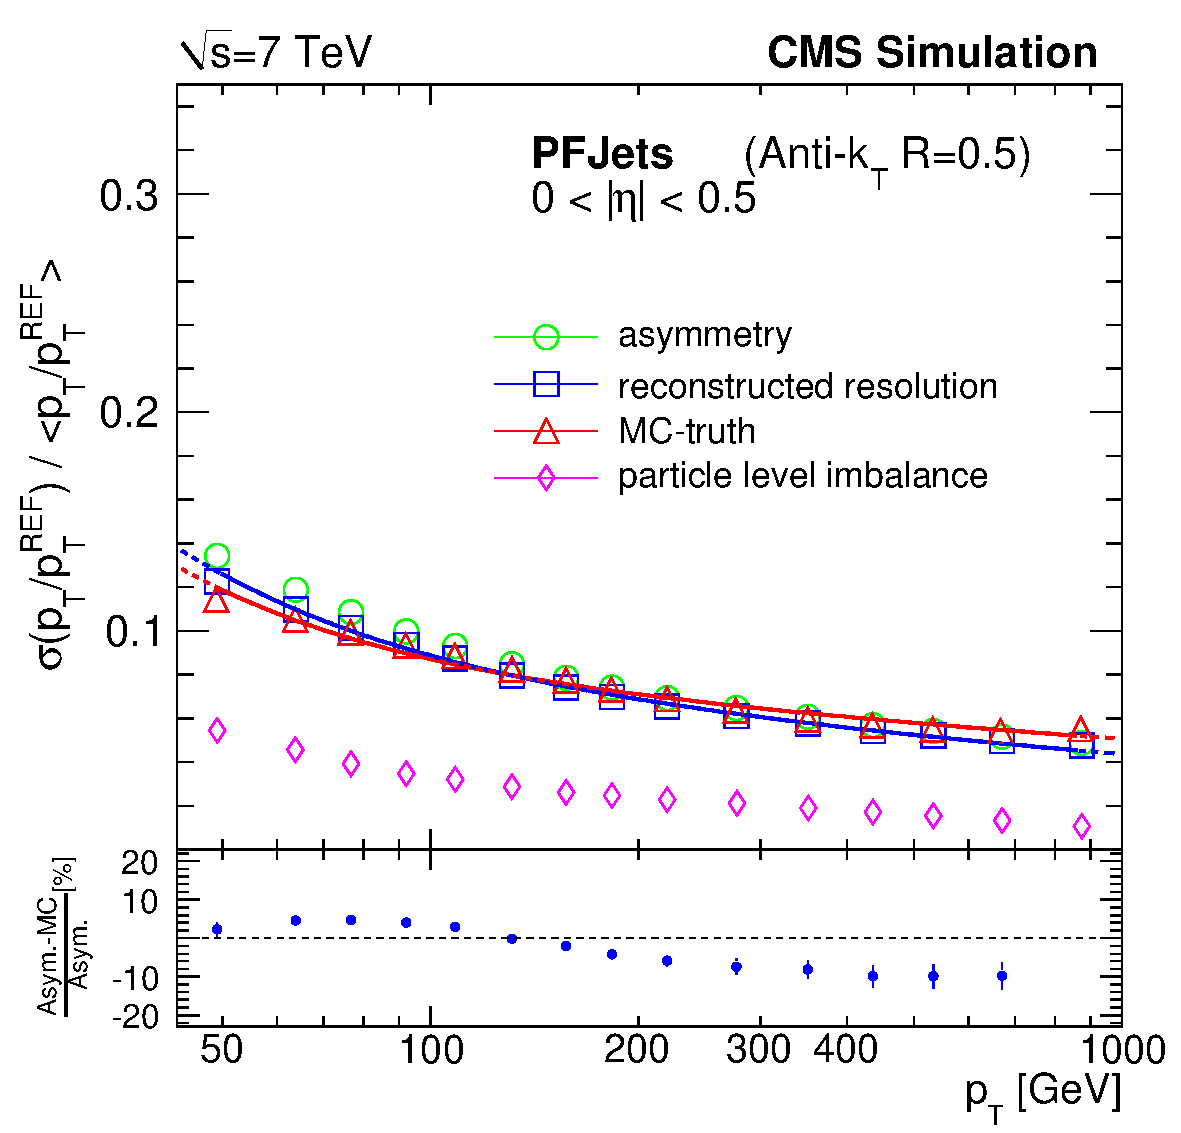
\includegraphics[width=0.45\textwidth]{Figures/JER/figs/res_dijet/ak5pf_mctruth_RelResVsRefPt_JetEta0to0dot5}
  \caption{Application of the asymmetry method to simulated CALO (top left), JPT (top right), and PF jets (bottom) in $|\eta|<0.5$.
The reconstruction-level (green circle) and particle-level (magenta diamond) results are shown together with the final measurement (blue square), compared to the generator-level MC (denoted as MC-truth) derived resolution (red triangle).}
  \label{fig:reso-mc-00to05}
\end{figure}

Several sources of systematic uncertainties are identified:

The linear extrapolation at half-the-distance between the standard working point (at $\ptrelthree=0.15$) and zero is evaluated, and the difference from the full extrapolation to zero is assigned as an uncertainty. The size of the particle-level imbalance is varied by $25\%$ and the impact of the measurement is studied when subtracting $75\%$ and $125\%$ of the original particle jet \pt resolution in quadrature.

Performing the analysis on simulated events, we observe deviations (biases) from the obtained and expected values, referred to as ``MC
closure  residuals''. A conservative $50\%$ of the MC closure residuals
$\frac{\mathrm{MC}(\mathrm{generator-level})-\mathrm{MC}(\mathrm{asymmetry})}{\mathrm{MC}(\mathrm{asymmetry})}$
is taken as an additional relative systematic uncertainty, corresponding to the bias correction. By comparing the asymmetry measured in data with the expectation from MC simulations, an  additional constant term is fitted, describing the observed discrepancy  between data and simulation, as  described below. The statistical  uncertainty from the  fit of the constant term is assigned as a systematic uncertainty. Figure~\ref{fig:urel-mc-00to05} shows the size of the different systematic uncertainties as a function of \ptave and for a central $\eta$ bin, for the three jets types. The particle-level imbalance uncertainty is shown in opaque orange, the solid yellow contribution corresponds to the uncertainty from the soft radiation variation, and the dashed-red line depicts the impact from the remaining differences in the MC closure. The relative uncertainty due to particle-level imbalance is larger for JPT and PF jets than for CALO jets because the absolute values of the raw resolutions are significantly smaller for JPT and PF, and thus more sensitive to the imbalance subtraction, than in the CALO jet case. The dashed blue line shows the contribution of the uncertainty on the additional constant term. The total systematic uncertainty for each resolution measurement is obtained by summing all individual components in quadrature, and is represented by the grey filled area in Fig.~\ref{fig:urel-mc-00to05}. The sensitivity of the method to the presence of additional collisions due to pile-up has been assessed by applying the measurement to the subsample of the data where exactly one primary vertex candidate is reconstructed, and no significant deviations from the inclusive measurement are observed.

\begin{figure}[h]
  \centering

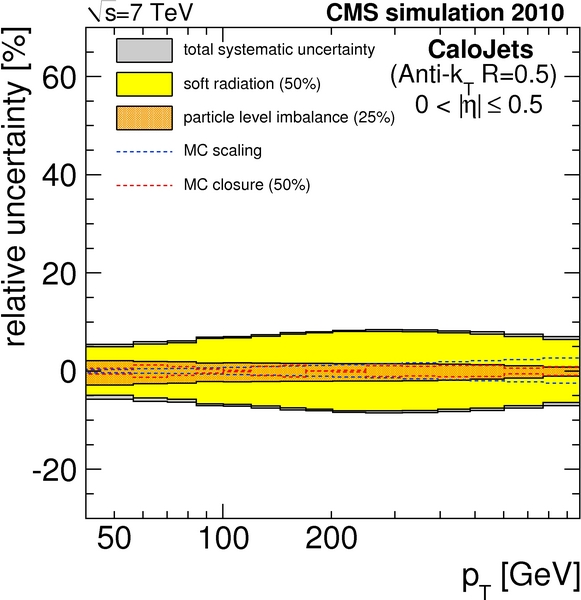
\includegraphics[width=0.45\textwidth]{Figures/JER/figs/res_dijet/urel_ak5calo_RelResVsRefPt_JetEta0to0dot5}
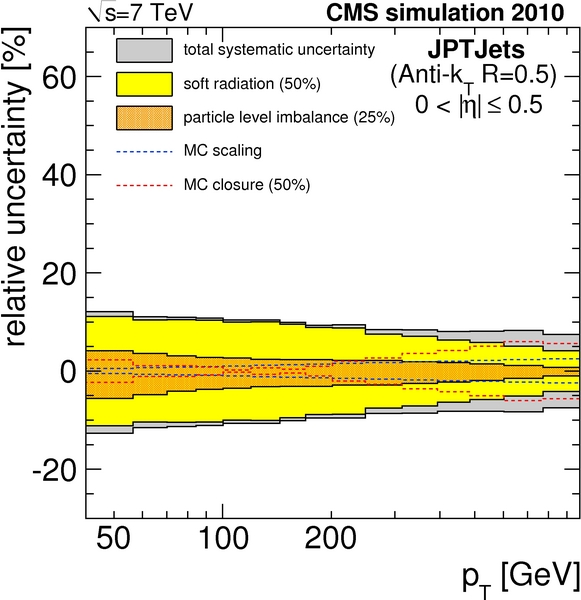
\includegraphics[width=0.45\textwidth]{Figures/JER/figs/res_dijet/urel_ak5jpt_RelResVsRefPt_JetEta0to0dot5}
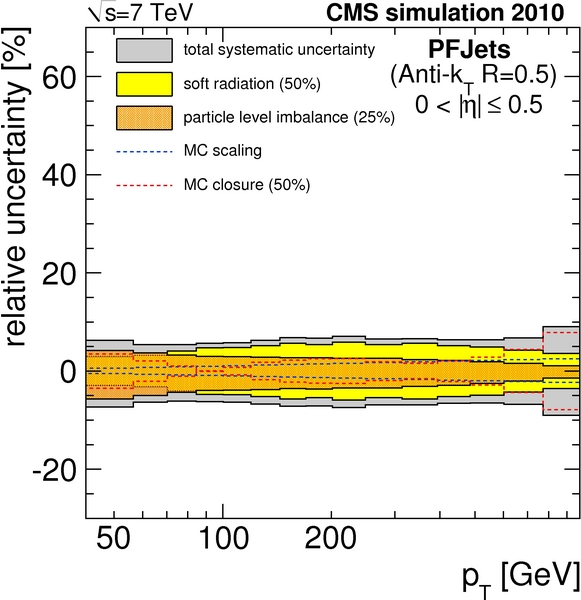
\includegraphics[width=0.45\textwidth]{Figures/JER/figs/res_dijet/urel_ak5pf_RelResVsRefPt_JetEta0to0dot5}
  \caption{Relative systematic uncertainty of the asymmetry method to simulated CALO (top left), JPT (top right), and PF jets (bottom) for $|\eta|<0.5$.}
  \label{fig:urel-mc-00to05}
\end{figure}

The presented measurements of the jet \pt resolution, obtained by applying
the asymmetry method to data, yield systematically poorer resolution
compared  to the simulation. This discrepancy is quantified by taking the
fits to the MC asymmetry results, fixing all parameters, and adding in quadrature an additional constant term, as the only free parameter in a subsequent fit to the data asymmetry. The fitted additional constant term provides a good characterization of the discrepancy, which was verified by several closure tests based on MC. A likely source of the discrepancy is an imperfect intercalibration of the CMS calorimeters, which affects analyses based on the corresponding datasets.

The final results are presented in Figs.~\ref{fig:uabs-mcdata-00to05} (for all three types of jets, in the central region) and \ref{fig:uabs-mcdata-05to50} (for PF jets in all remaining $\eta$ bins). In each case, the solid red line depicts the resolution from generator-level MC, corrected for the measured discrepancy between data and simulation (constant term), and represents the best estimate of the jet \pt resolution in data. Consequently, it is central to the total systematic uncertainty band, drawn in yellow. The uncorrected generator-level MC resolution is shown as a red-dashed line for reference. The black dots are the bias-corrected data measurements, which are found to be in good agreement with the discrepancy-corrected  generator-level MC, within the statistical and systematic uncertainties. Note in particular that the agreement with the uncorrected generator-level MC resolution is considerably worse.

\begin{figure}[h]
  \centering
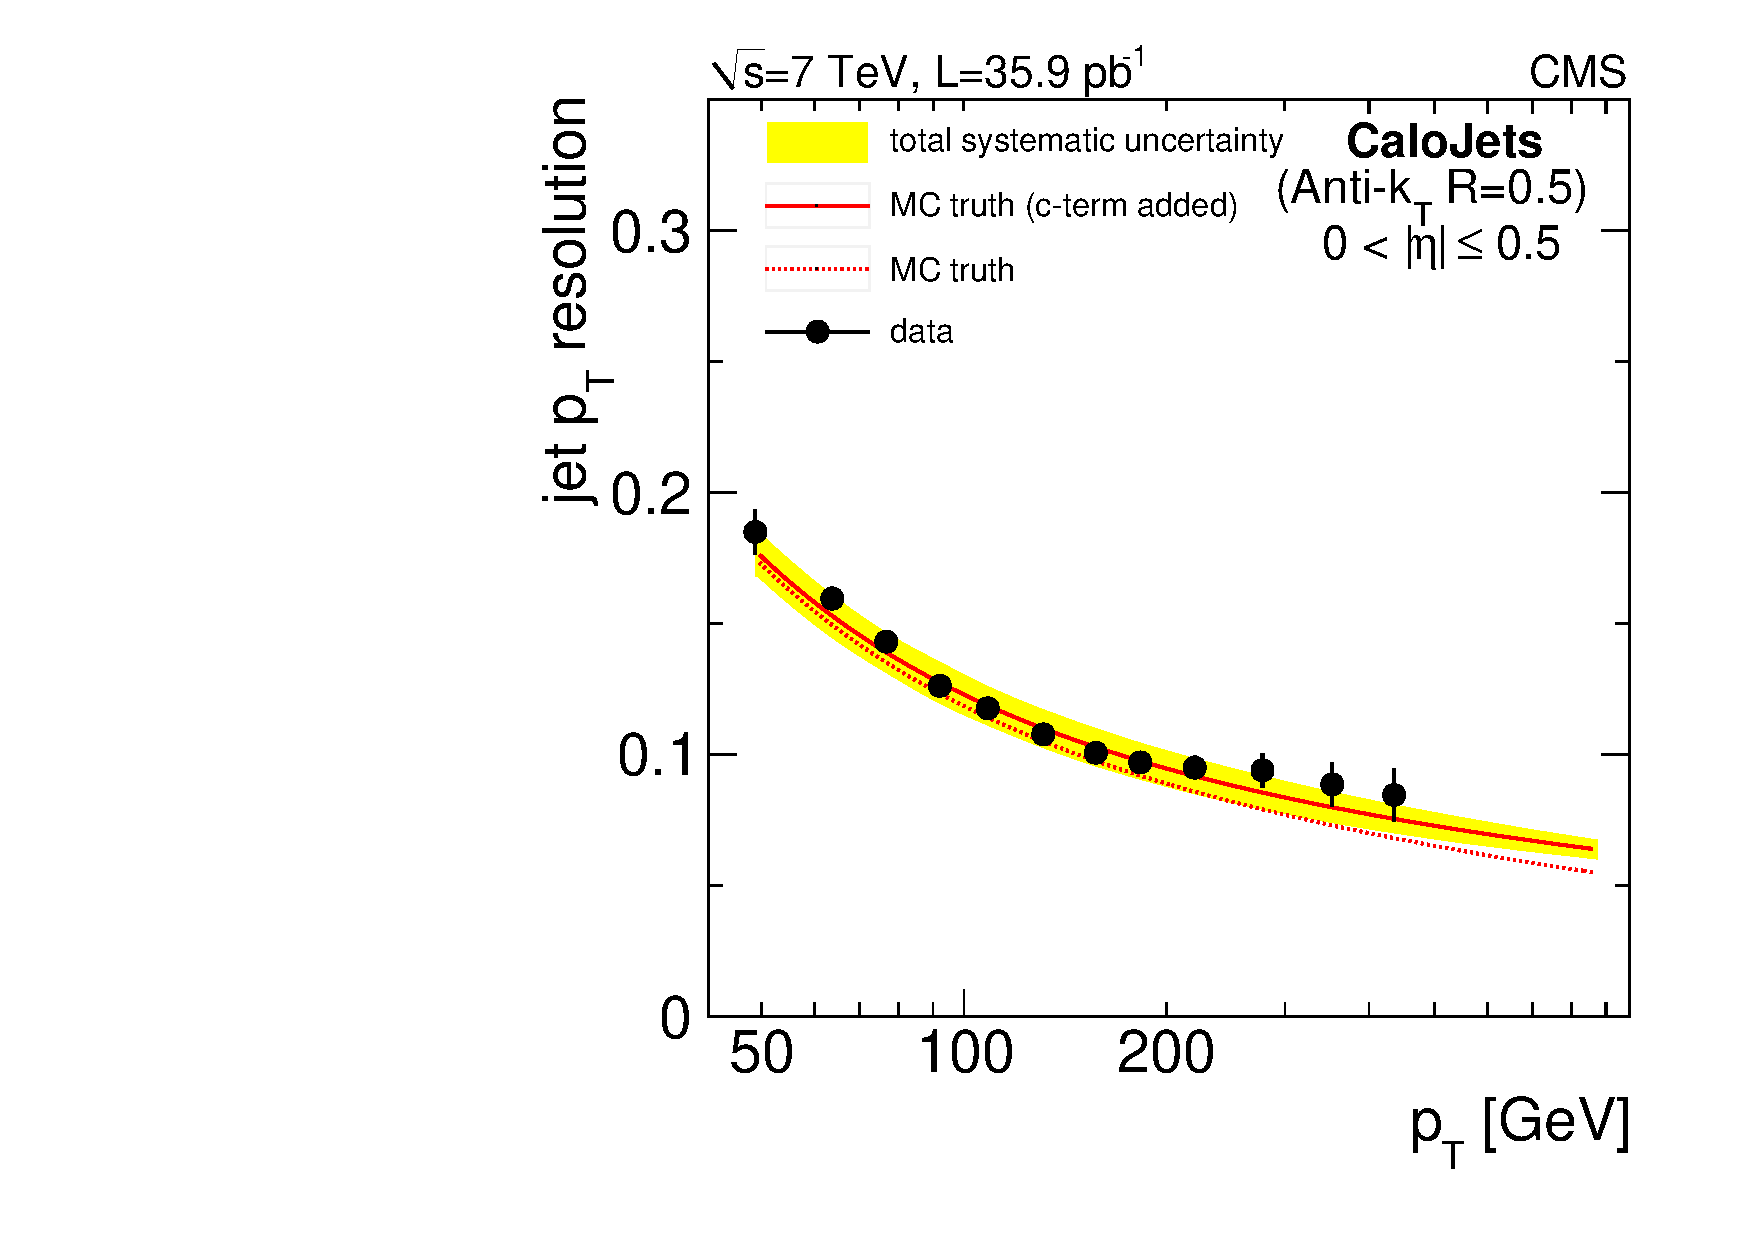
\includegraphics[width=0.45\textwidth]{Figures/JER/figs/res_dijet/uabs_ak5calo_RelResVsRefPt_JetEta0to0dot5}
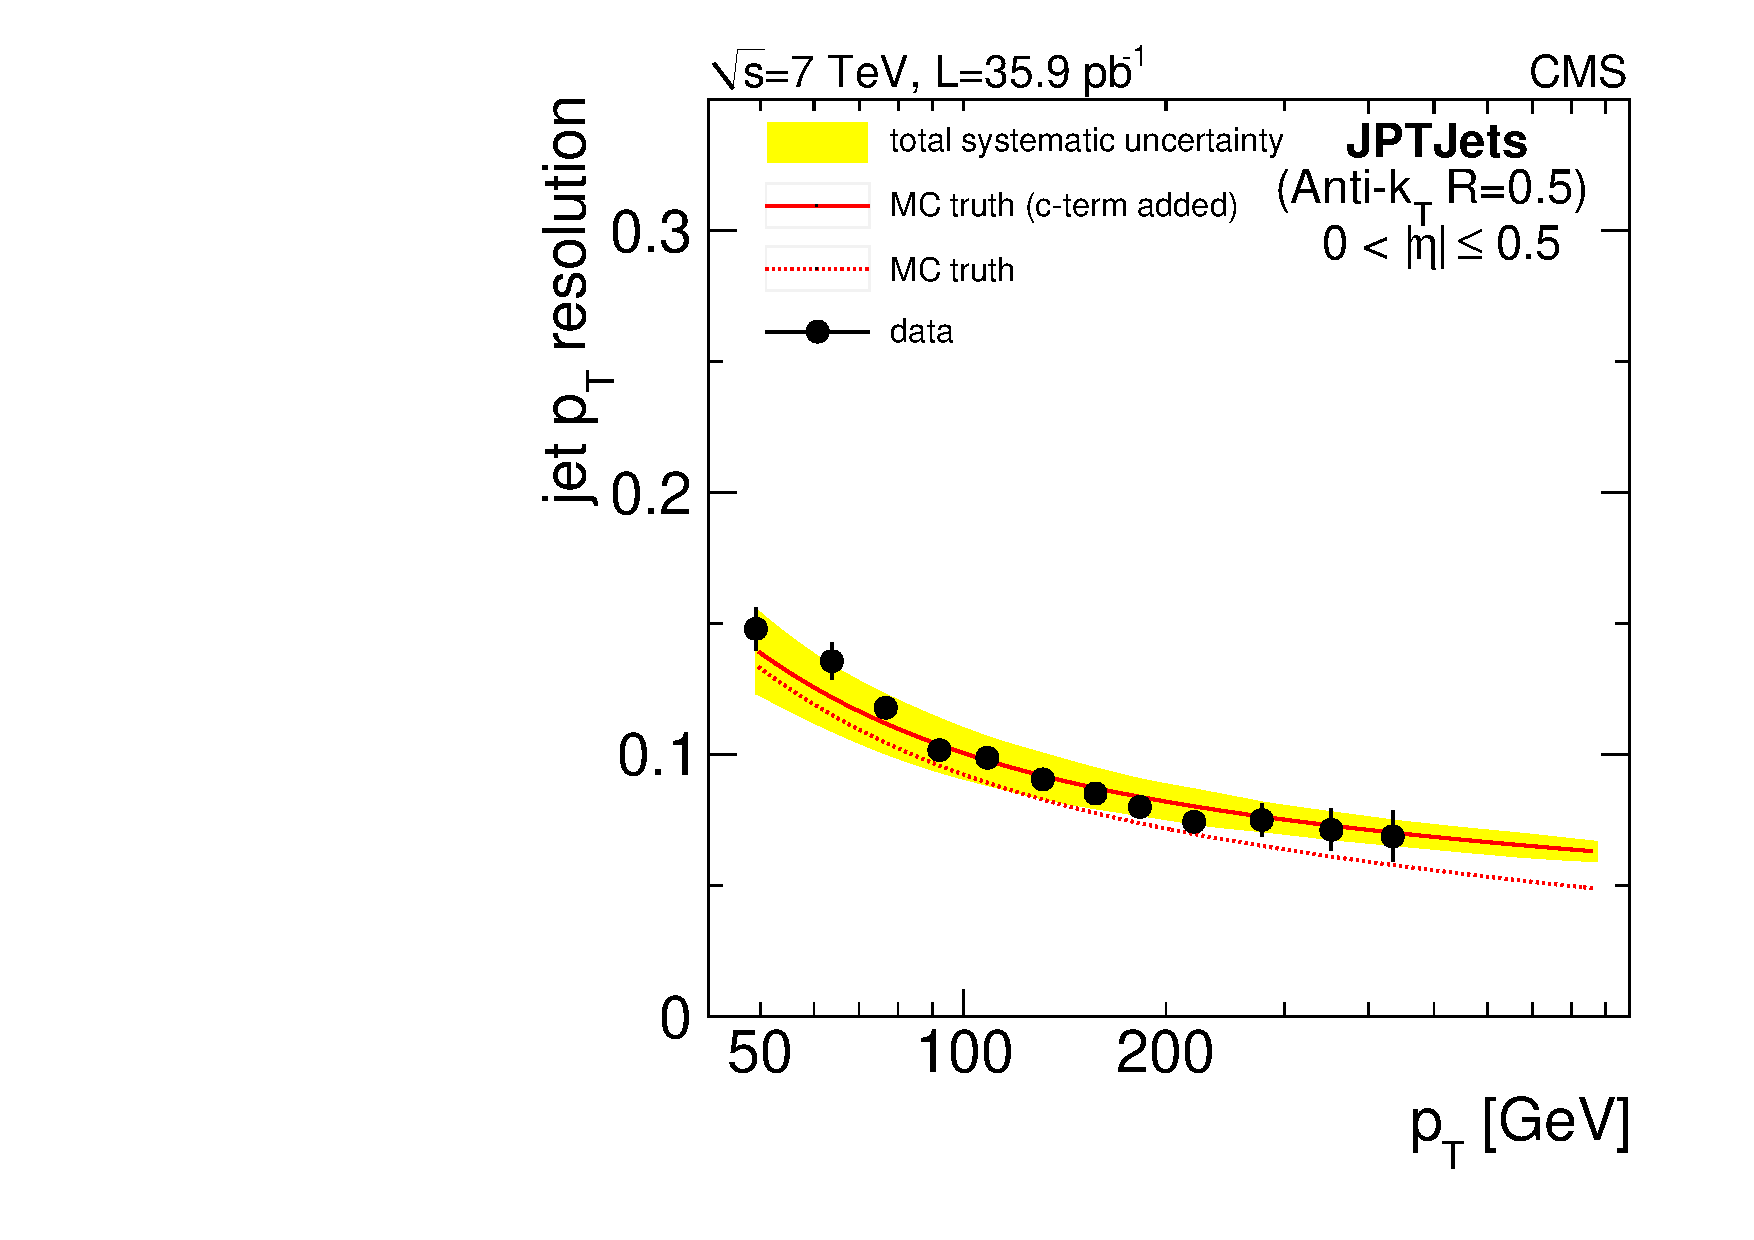
\includegraphics[width=0.45\textwidth]{Figures/JER/figs/res_dijet/uabs_ak5jpt_RelResVsRefPt_JetEta0to0dot5}
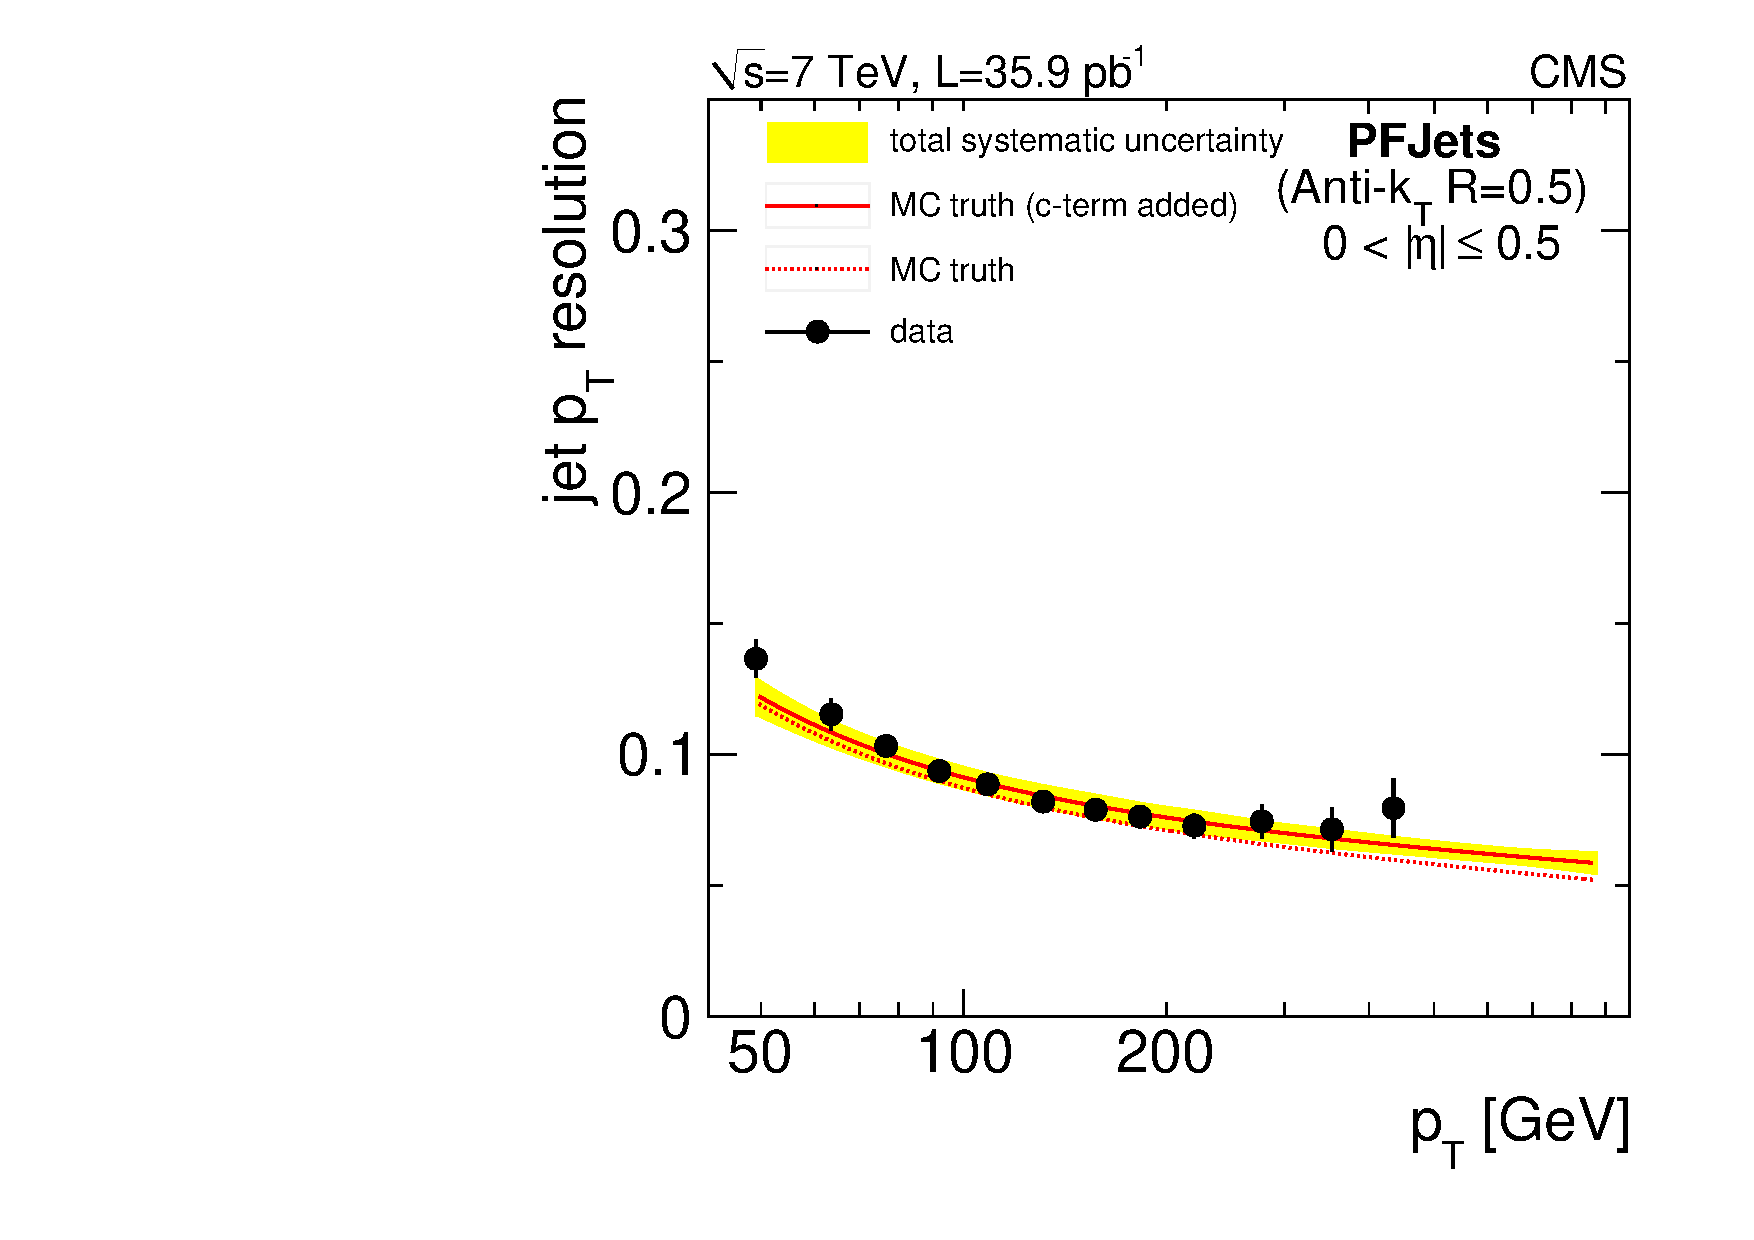
\includegraphics[width=0.45\textwidth]{Figures/JER/figs/res_dijet/uabs_ak5pf_RelResVsRefPt_JetEta0to0dot5}
  \caption{Bias-corrected data measurements, compared to the generator-level MC (denoted as MC-truth) \pt resolution before (red-dashed line) and after correction for the measured discrepancy between data and simulation (red-solid line) for CALO (top left), JPT (top right), and PF jets (bottom) in $|\eta|<0.5$.}
  \label{fig:uabs-mcdata-00to05}
\end{figure}

\begin{figure}[h]
  \centering

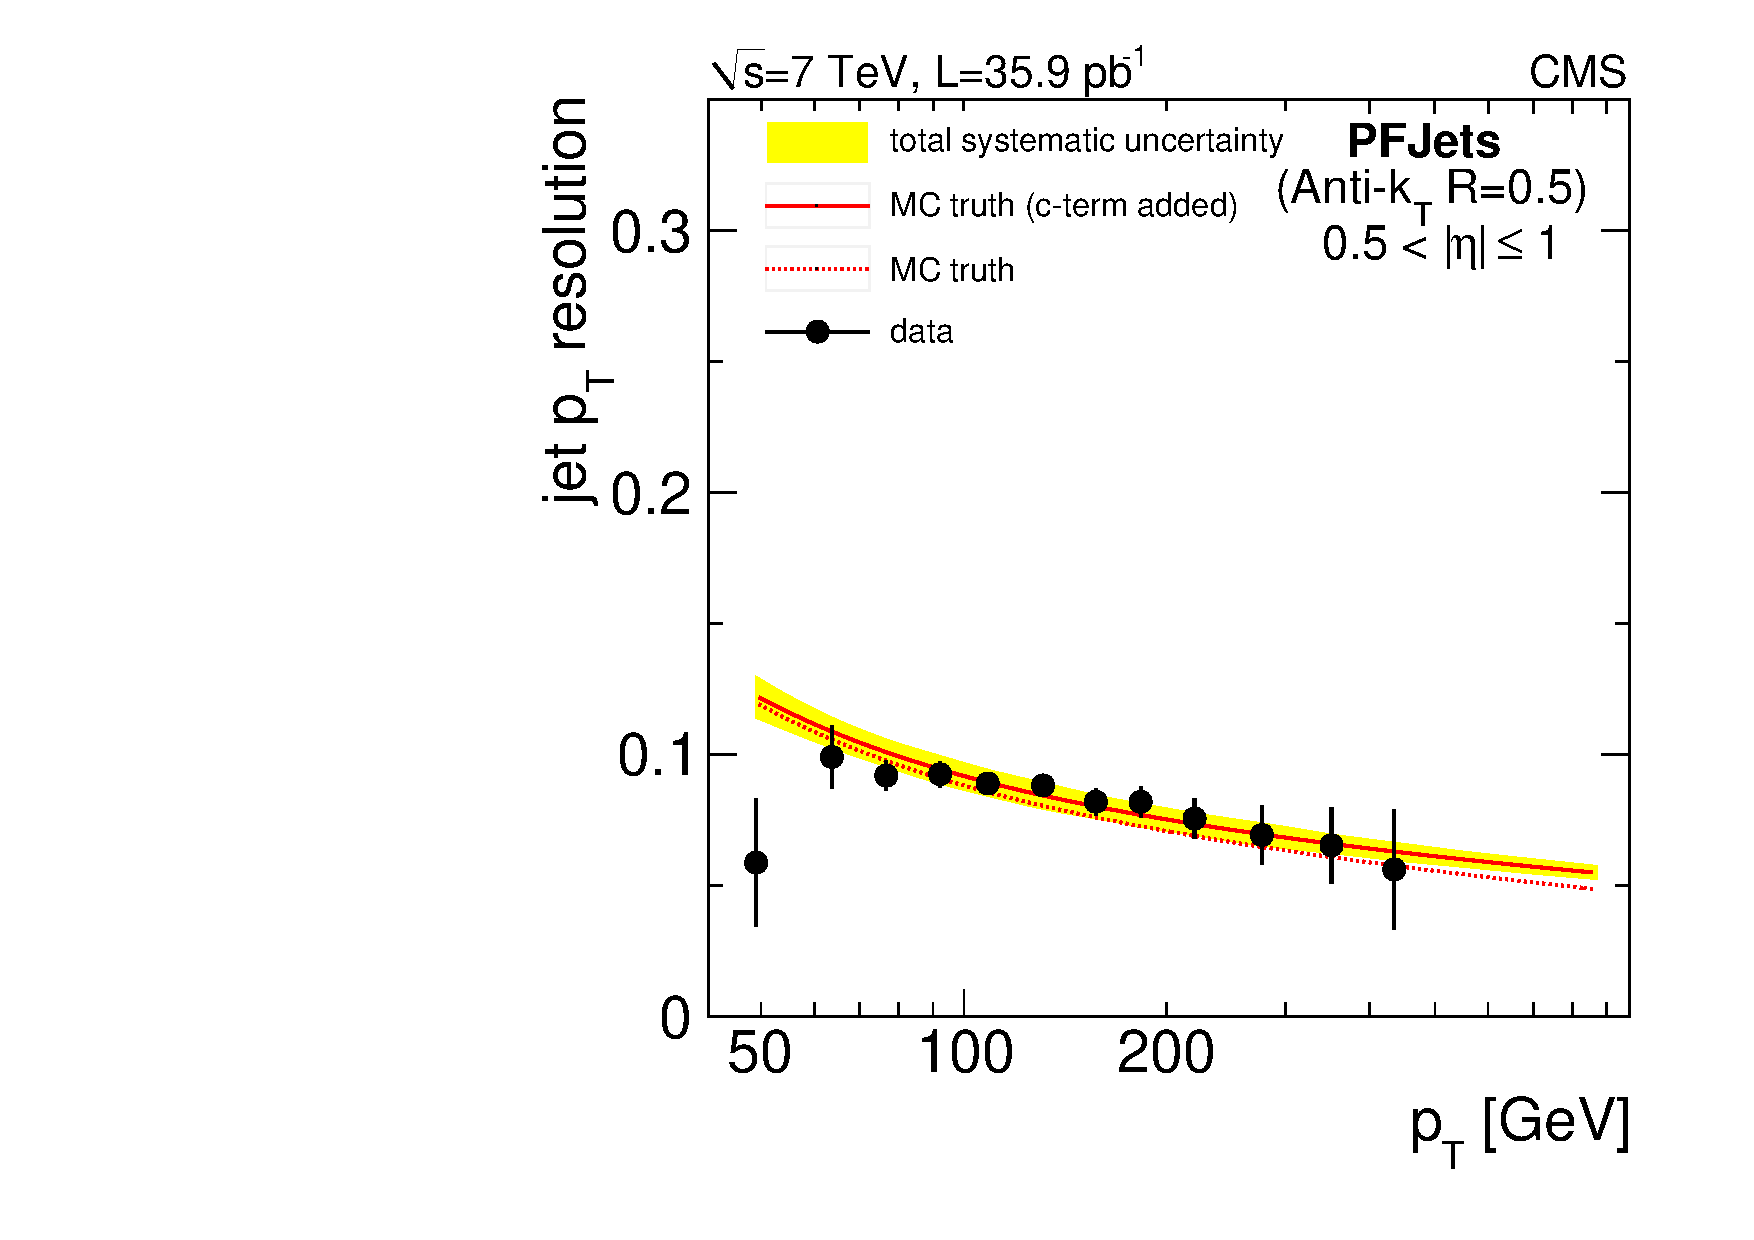
\includegraphics[width=0.45\textwidth]{Figures/JER/figs/res_dijet/uabs_ak5pf_RelResVsRefPt_JetEta0dot5to1}
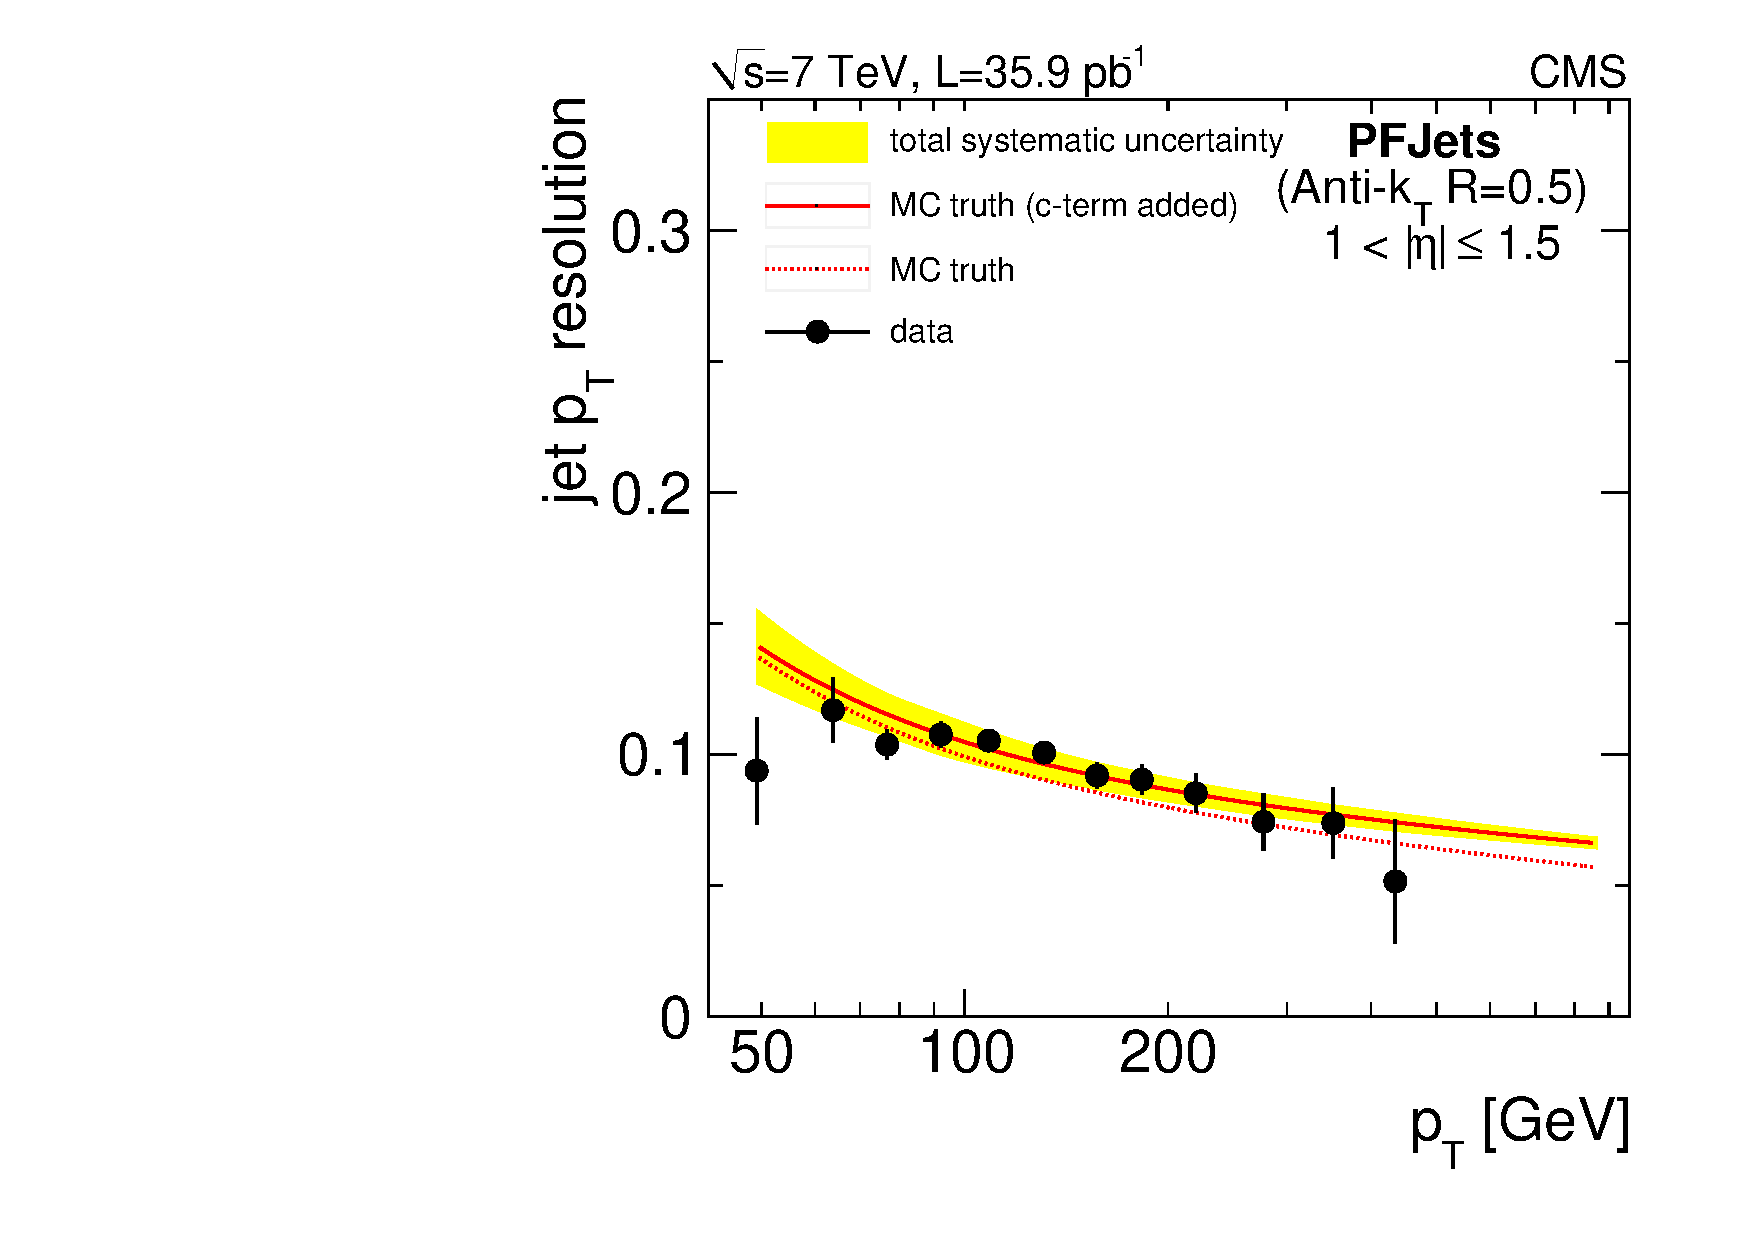
\includegraphics[width=0.45\textwidth]{Figures/JER/figs/res_dijet/uabs_ak5pf_RelResVsRefPt_JetEta1to1dot5}
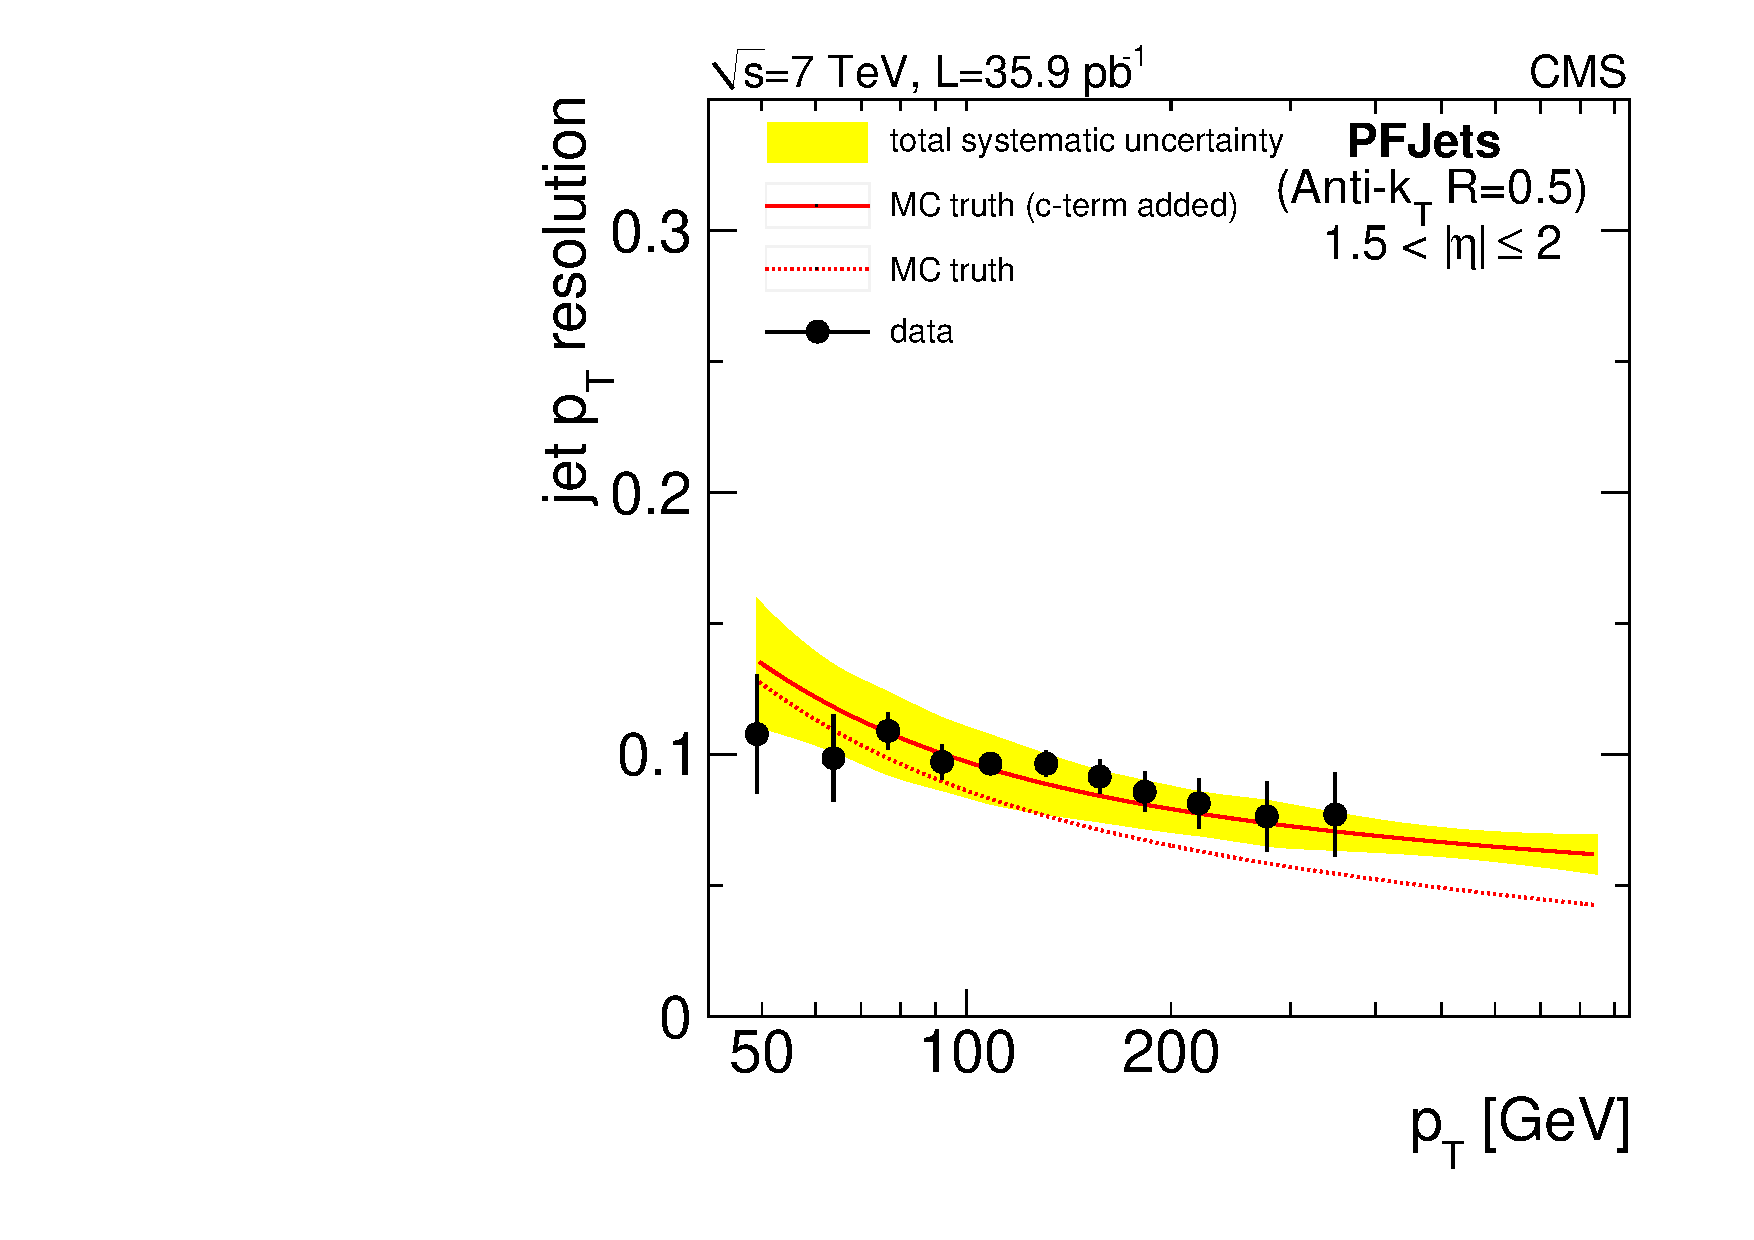
\includegraphics[width=0.45\textwidth]{Figures/JER/figs/res_dijet/uabs_ak5pf_RelResVsRefPt_JetEta1dot5to2}
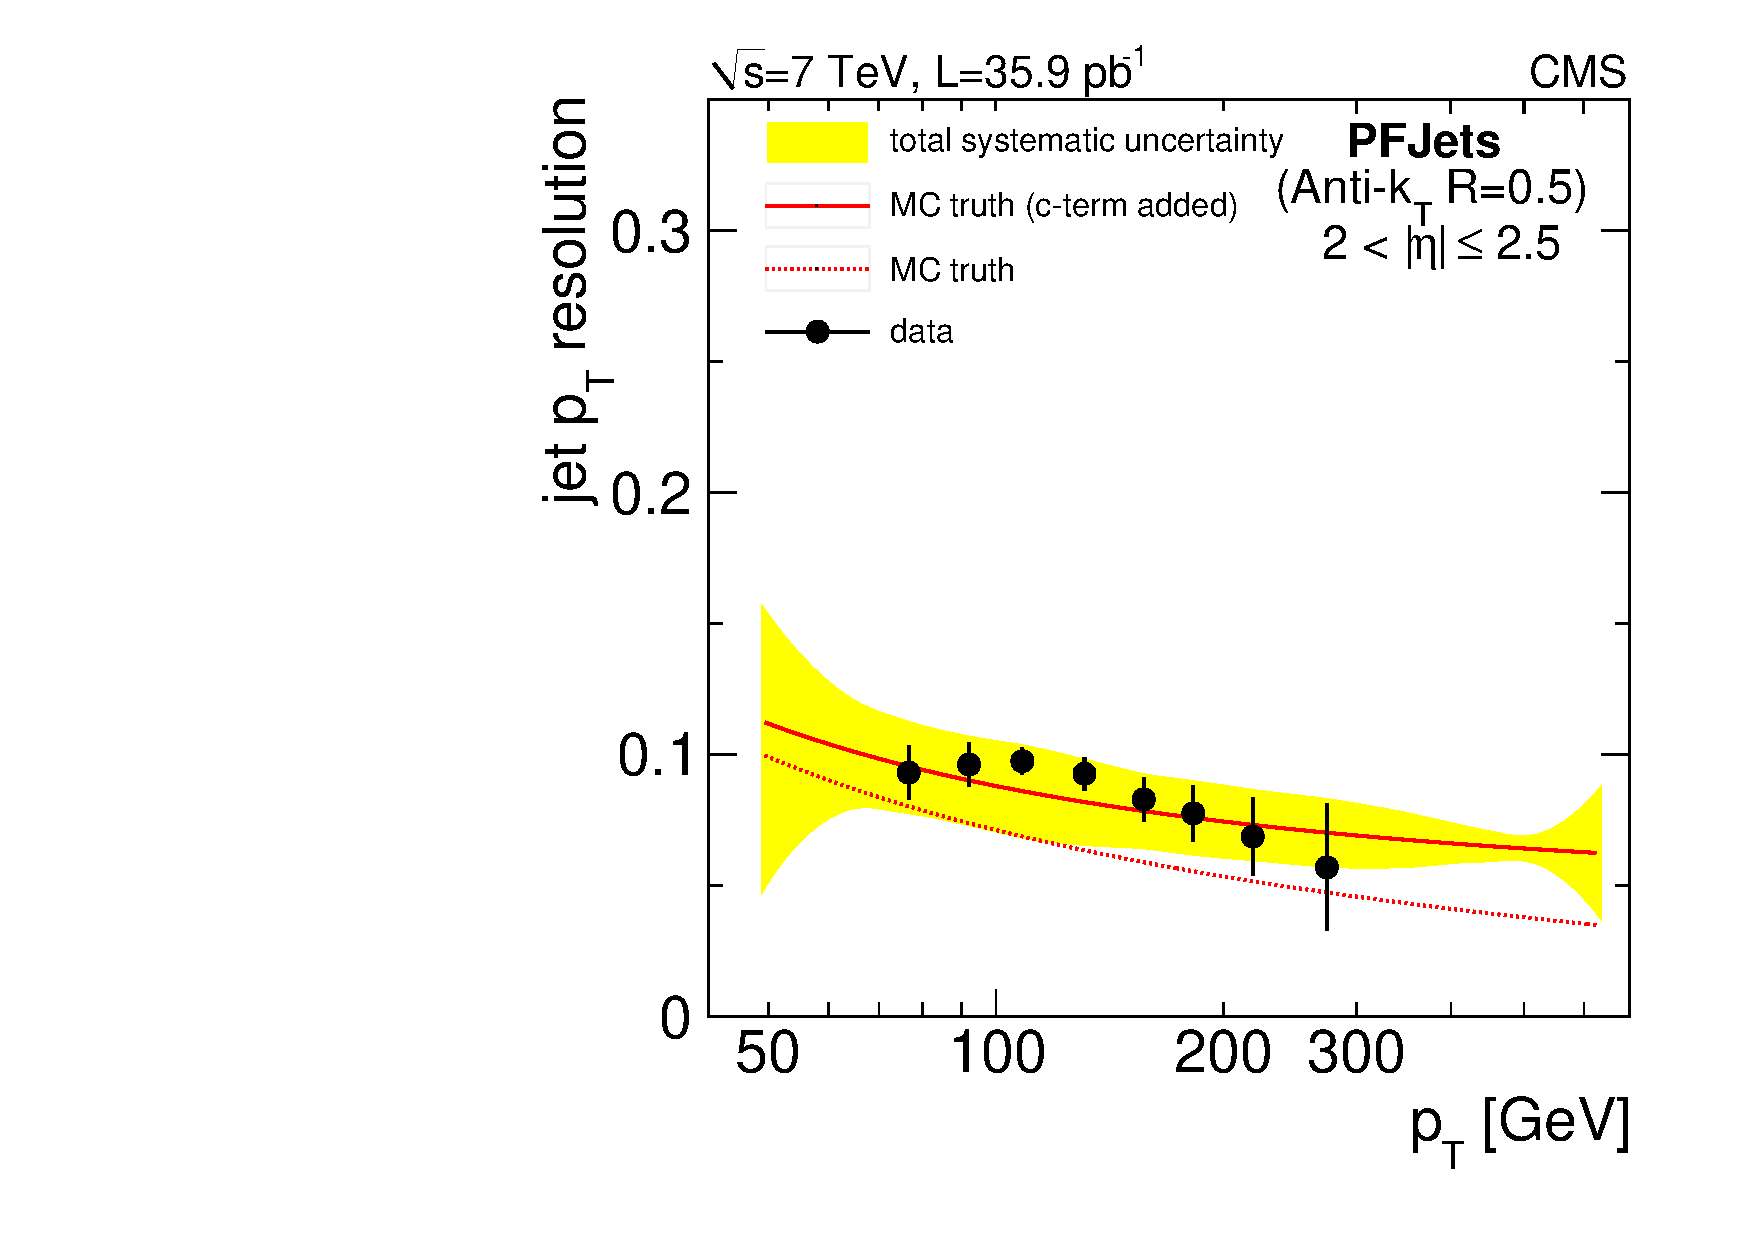
\includegraphics[width=0.45\textwidth]{Figures/JER/figs/res_dijet/uabs_ak5pf_RelResVsRefPt_JetEta2to2dot5}
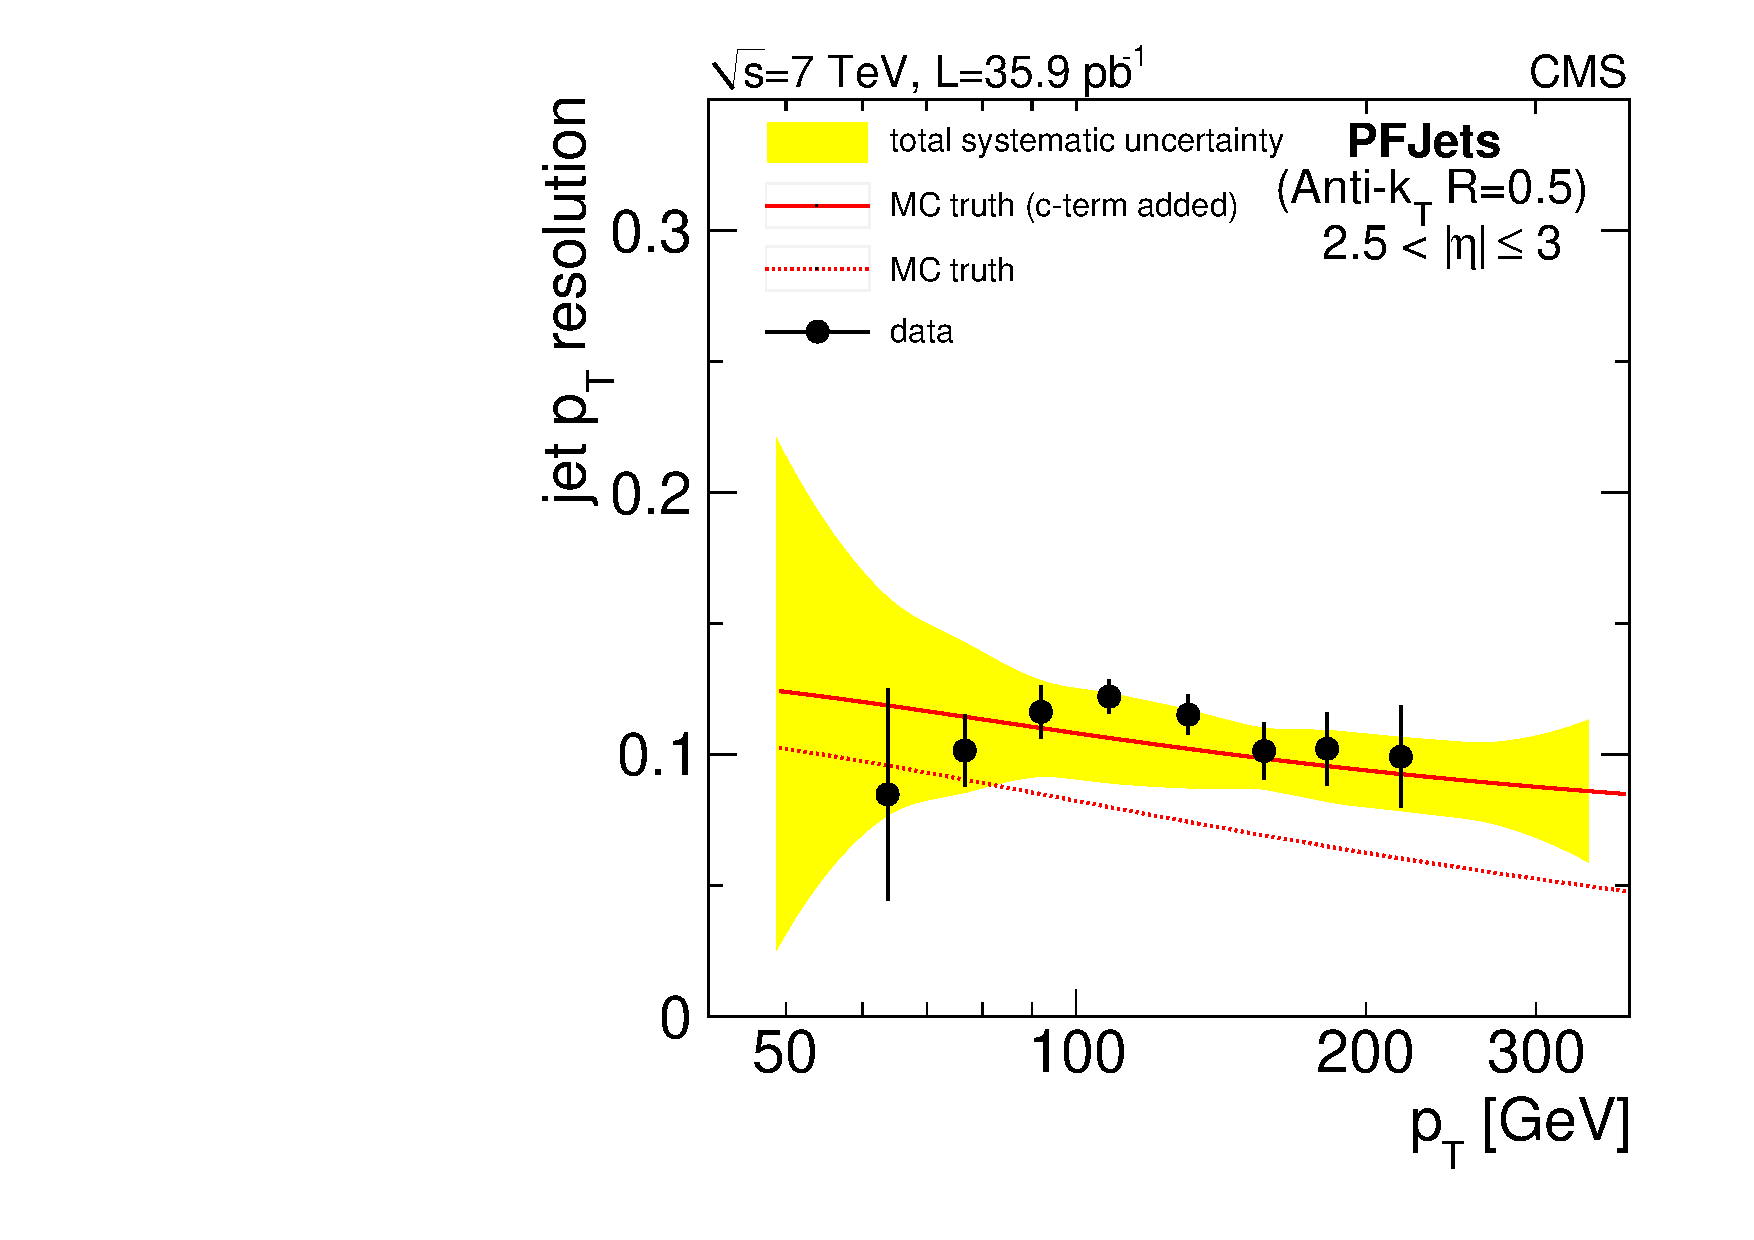
\includegraphics[width=0.45\textwidth]{Figures/JER/figs/res_dijet/uabs_ak5pf_RelResVsRefPt_JetEta2dot5to3}
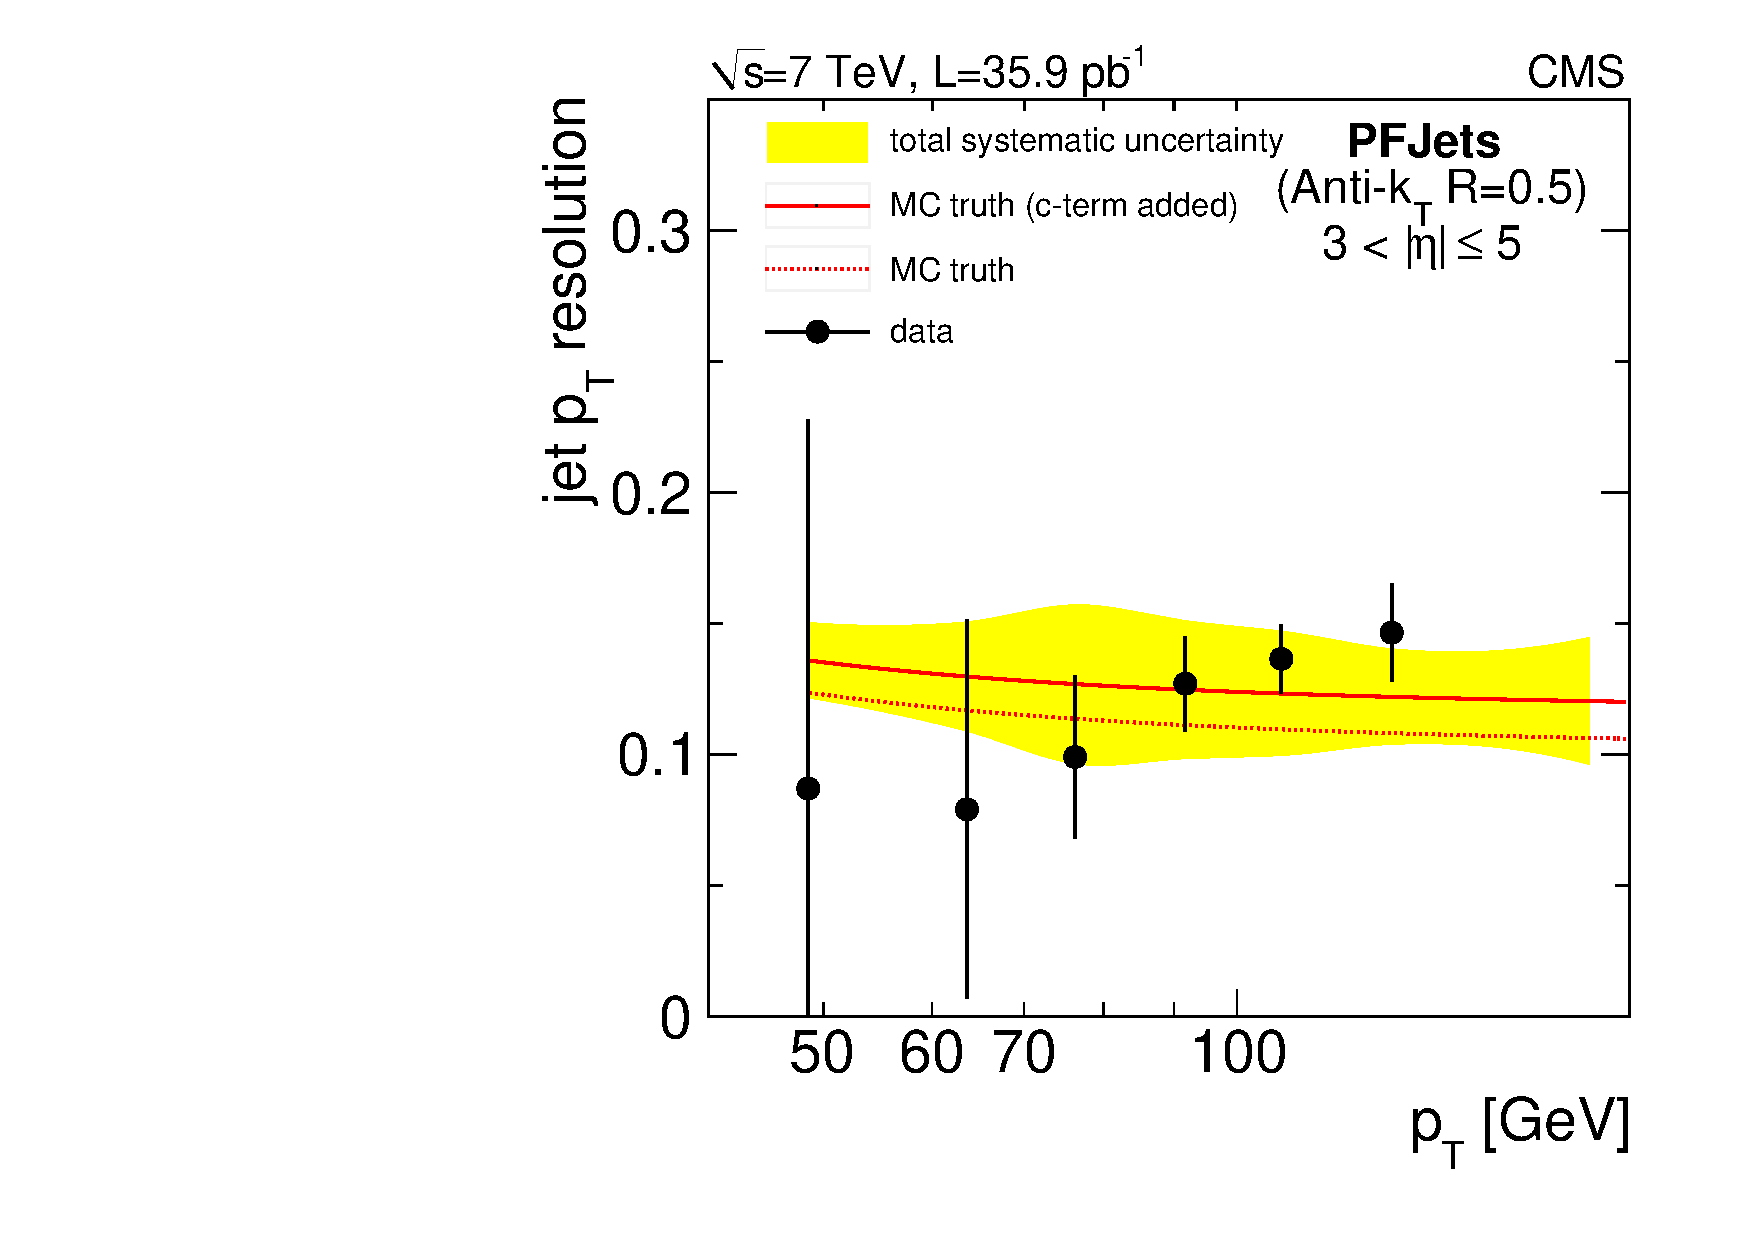
\includegraphics[width=0.45\textwidth]{Figures/JER/figs/res_dijet/uabs_ak5pf_RelResVsRefPt_JetEta3to5}
  \caption{Bias-corrected data measurements, compared to the generator-level MC (denoted as MC-truth) resolution before (red-dashed line) and after correction for the measured discrepancy between data and simulation (red-solid line), compared to data, for PF jets in different $\eta$ ranges.}
  \label{fig:uabs-mcdata-05to50}
\end{figure}

The dijet data are also investigated within the framework of the unbinned likelihood fit to the jet \pt resolution parameterization. This approach is developed in order to provide a cross-check of the results. It also serves  as a tool for the determination of the full jet \pt resolution  function, once larger collider data samples become available. This method directly takes into account biases in the event selection caused by the jet \pt resolution and the steeply falling jet \pt spectrum.

At the present stage, the jet \pt probability densities are approximated
by a truncated Gaussian, providing direct correspondence with the binned
fits discussed above. The resulting determination of the widths of the jet
\pt resolution (as function of \pt and $\eta$) is also affected by the
soft-radiation and hadronization (out-of-cone) effects. The fitted
resolution values are thus extrapolated to zero-radiation activity. The MC
particle-level imbalance is subtracted in quadrature to correct for
effects of hadronization. The method is applied to both data and MC, and
the results are consistent with the previously discussed binned fits to
the asymmetry distributions. Namely, poorer resolutions are observed in
data compared to the simulation.

